\documentclass[12pt]{article}

\usepackage{booktabs}
\usepackage{dcolumn} 
\usepackage{epstopdf}
\usepackage{graphicx}
\usepackage{hyperref}
\usepackage{longtable} 
\usepackage{natbib}
\usepackage{rotating}
\usepackage{tabularx}
\usepackage{amsmath}
\usepackage{setspace}
\usepackage{caption}

\usepackage[super]{nth}  
\hypersetup{
  colorlinks = TRUE,
  citecolor=blue,
  linkcolor=red,
  urlcolor=black
}

\hypersetup{colorlinks = TRUE, citecolor=blue, linkcolor=red, urlcolor=black}

\DeclareMathOperator*{\argmax}{arg\,max}

\newcommand{\starlanguage}{Significance indicators: $p \le 0.05:*$, $p \le 0.01:**$ and $p \le .001:***$.}

\newcommand{\covid}{Covid-19}  

\newtheorem{proposition}{Proposition}
\newtheorem{assumption}{Assumption}
\newtheorem{example}{Example}
\newtheorem{observation}{Observation}
\newtheorem{lemma}{Lemma}

\newcommand{\important}[1]{\textcolor{blue}{\textbf{ #1}}}
\newcommand{\quantclaim}[1]{\textcolor{red}{\textbf{ #1}}}


\newcommand{\LFPRhat}{58}
\newcommand{\numObs}{4,946}
\newcommand{\numObsWorking}{2,845}
\newcommand{\SurveyStart}{2020-06-29}
\newcommand{\SurveyEnd}{2020-07-04}
\newcommand{\LaidOff}{8.0}
\newcommand{\LaidOffLB}{4.5}
\newcommand{\LaidOffUB}{11.5}
\newcommand{\WFH}{28.4}
\newcommand{\WFHLB}{25.3}
\newcommand{\WFHUB}{31.5}
\newcommand{\alreadyWFH}{14.3}
\newcommand{\alreadyWFHLB}{10.9}
\newcommand{\alreadyWFHUB}{17.7}
\newcommand{\stillCommute}{42.7}
\newcommand{\stillCommuteLB}{40.0}
\newcommand{\stillCommuteUB}{45.5}


\begin{document} 

\title{Covid19 and Work-From-Home in the US:\\ An Early Look}

\date{\today}

\author{Erik Brynjolfsson\\Stanford \& NBER \and John Horton\footnote{
    MIT's COUHS ruled this project as expempt (number E-2075). 
  }\\MIT \& NBER \and Adam Ozimek\\Upwork \and Daniel Rock\\MIT \and Garima Sharma\\MIT \and Hong Yi Tu Ye\\MIT}

\maketitle

\begin{abstract}
  \noindent The on-going \covid{} pandemic has confined large numbers of people to their homes and caused unprecedented lay-offs.
  Of those previously employed, \LaidOff{}\% (95\% CI is [\LaidOffLB,\LaidOffUB]), report being laid-off our furloughed in the last 4 weeks.
  Among the same sample, \WFH{}\% (95\% CI is [\WFHLB,\WFHUB]), they were previously commuting and are now working from home.
  The percentage already working from home pre-Covid-19 is \alreadyWFH{}\% (95\% CI is [\alreadyWFHLB,\alreadyWFHUB]). 
  We document substantial geographic variation in responses, particularly with the fraction now working from home. 
%  The timing of singups is consistent with 
  \newline 
%% \noindent JEL J01, J24, J3 \newline 
%% keywords: bargaining, match formation, wage determination
\end{abstract} 

\onehalfspacing 

\section{Introduction}
The on-going \covid{} pandemic has confined large numbers of people to their homes via quarantines and shelter-in-place orders.
Large numbers of businesses are closed. 
There have already been enormous and unprecedented increases in workers filing unemployment insurance claims \citep{goldsmith2020}. 
To get a real-time sense of how firms and workers are responding, we conducted a Google Consumer Surveys (GCS). 
We asked a single question:
````Have you started to work from home in the last 4 weeks?''
with the following response options: 
\begin{enumerate} 
\item ``I continue to commute to work''
\item ``I have recently been furloughed or laid-off''
\item ``Used to commute, now work from home''   
\item ``Used to work from home and still do''       
\item ``Used to work from home, but now I commute''
\item ``None of the above / Not working for pay''
\end{enumerate} 

We launched our survey on \SurveyStart{}; this report includes responses up until \SurveyEnd{}. 
So far, we have surveyed a total of \numObs{} respondents.

\section{Results}

Of the respondents, \numObsWorking{} reported something other than ``None of the above / Not working for pay.''
This gives an implied employment rate of \LFPRhat{}\%, which is slightly lower than the BLS estimate of about 60\%.\footnote{
  \url{https://fred.stlouisfed.org/series/EMRATIO}
}
We restrict our sample those reporting being employed 4 weeks prior.

The distribution of answers pooled over all respondents is shown in Figure~\ref{fig:working_summary}. 
We can see that the most common response from workers was that they continue to commute, at \stillCommute{}\% (95\% CI is [\stillCommuteLB,\stillCommuteUB]). 
But the next most common was that they were now working from home. 

The \emph{now} working from home fraction is about \WFH{}\%.
\cite{dingel2020} that 34\% of jobs in the US can plausibly be performed from home. 
However, we a substantial fraction were already working from home in they survey: \alreadyWFH{}\% reporting they were already working from home pre-Covid-19.
The ATUS release has 23.7\% working from home on an average day, though our question implies working from home all the time; the from home only fraction in the ATUS is 18.2\%. 
Our \WFH{}\% is also broadly consistent with the ``Freelancing in American Survey'' that reported 16.8\% report doing most of all of their work remote \citep{upwork2019}, though this included people working from co-working spaces, coffee shomes, homes and so on.
The Census 2019 gives 5.3\% as ``working from home some'' so there is clearly lot of respondent uncertainty about what precisely various questions mean. 
%The BLS reported fraction is TK. 

% As we will see, there is some regional variation, though we make no attempt to account for differing regions having different job compositions.



% upwork2019,

If we take the US labor force at about 165M, with an 11\% increase in furloughs/lay-offs, the implication is about 16M Americans recently out of work.
The total UI filings for the last to weeks adds up to 9.9M.\footnote{
  \url{https://www.dol.gov/ui/data.pdf}
}
However, not all unemployed have yet filed for unemployment.
Given the decline in hiring, Prof. Wolfers estimates we are dealing with about 16M unemployed, which matches our point estimate.\footnote{
  \url{https://www.nytimes.com/2020/04/03/upshot/coronavirus-jobless-rate-great-depression.html}
}

% https://fred.stlouisfed.org/series/CLF16OV
%% This number makes total sense.  However, no everyone laid off applies for unemployment. And that data is only up through March 28. This number is very very plausible. In fact looking at all the UI data and also lower hiring rate, Wolfers estimates that we are dealing with 16 m so far, so you are like exactly on point 

\begin{figure}
  \caption{Answers to the question ``Have you started to work from home in the last 4 weeks?'', conditional upon being in the labor force from a US sample} \label{fig:working_summary}
\centering
\begin{minipage}{1.0 \linewidth}
  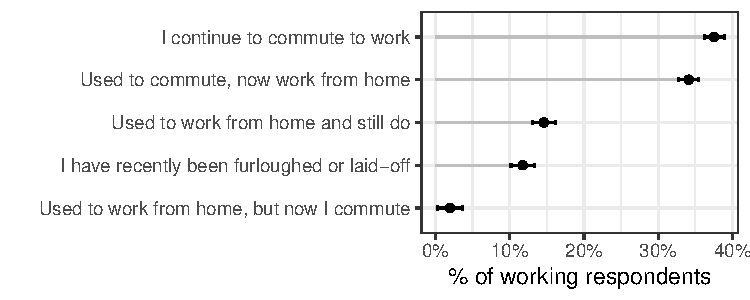
\includegraphics[width = \linewidth]{plots/working_summary.pdf} \\
  \begin{footnotesize}
    %% \begin{singlespace}
    %%   \emph{Notes:} 
    %% \end{singlespace}
    \end{footnotesize}
\end{minipage}
\end{figure} 

GCS also infers respondent gender.
We analyzed responses by gender but did not find any notable differences.
See Appendix~\ref{sec:gender} for this analysis. 

\subsection{Geographic variation} 
Covid-19 has affected different parts of the US differently, with the main epicenter being NYC. 
In Figure~\ref{fig:region}, we plot the fraction of respondents choosing each answer, by region.
GCS captures a respondents city and state, which are then mapped to the regions ``Northeast'', ``Midwest'', ``West'' and ``South.'' 

In the first facet from the left, we can see that the south has the highest fraction still commuting to work and the northeast has the lowest. 
In the second facet from the right, we can see that the northeast has the highest fraction of respondents switching to working from home, and the south the fewest.
The northeast started from the lowest fraction working from home, though these fractions are imprecisely estimated and are all fairly similar to each other. 
The northeast fraction now working from home is over 40\%, though the CI would just about reach the \cite{dingel2020} estimate.

\begin{figure}
  \caption{Responses by US region} \label{fig:region}
\centering
\begin{minipage}{1.0 \linewidth}
  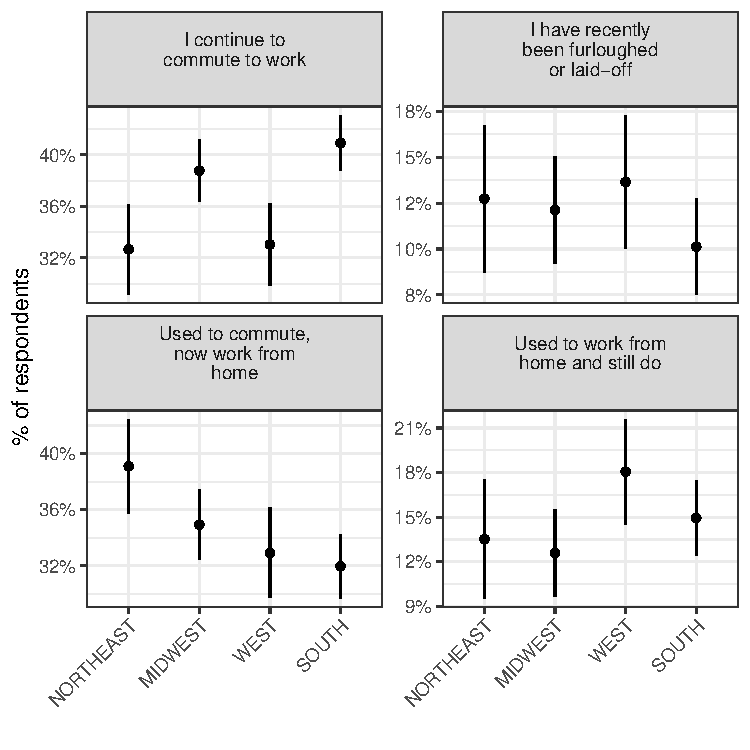
\includegraphics[width = \linewidth]{plots/region.pdf} \\
  \begin{footnotesize}
%    \begin{singlespace}
%      \emph{Notes:} Standard errors are reported. 
%    \end{singlespace}
    \end{footnotesize}
\end{minipage}
\end{figure} 

For a finer-grained look, we plot responses by state in Figure~\ref{fig:geo}.
It is important to keep in mind that some of these point estimates are fairly imprecise.

The fraction that are still continuing to commute to work is highest in the Dakotas, Wyoming and Montana.
There is still a substantial fraction in the south continuing to commute. 
The northeast, with the exception of Vermont, shows large reductions in people still commuting to work. 

\begin{figure}
  \caption{Responses by US State} \label{fig:geo}
\centering
\begin{minipage}{1.0 \linewidth}
  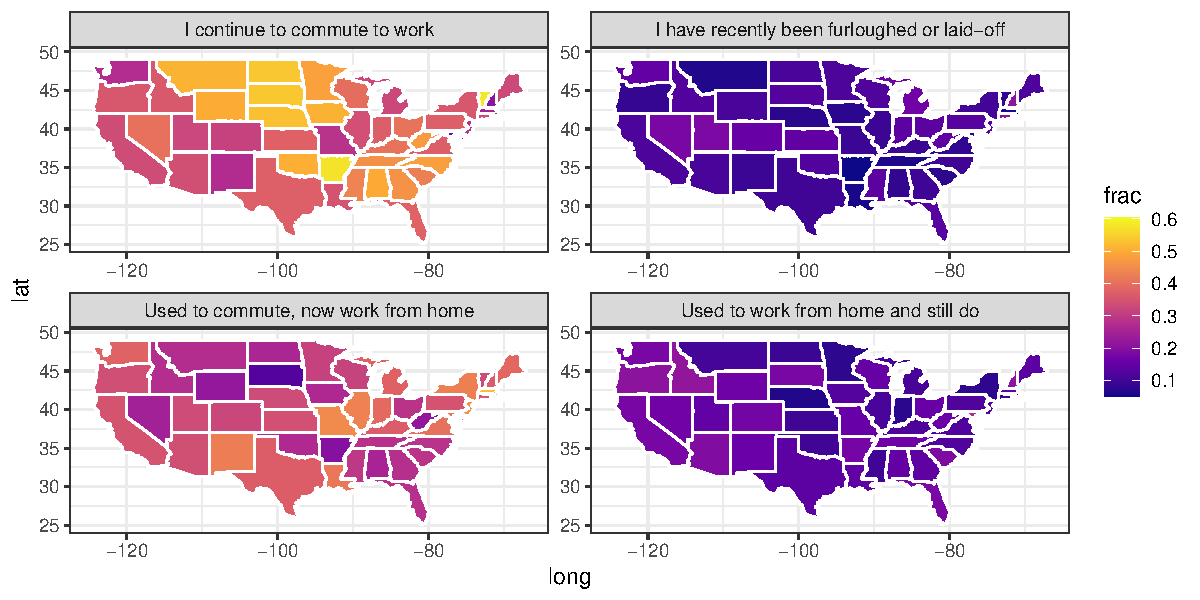
\includegraphics[width = \linewidth]{plots/geo.pdf} \\
  \begin{footnotesize}
    %% \begin{singlespace}
    %%   \emph{Notes:} 
    %% \end{singlespace}
    \end{footnotesize}
\end{minipage}
\end{figure} 

\section{Conclusion}
We document some early facts about how the US labor force is responding to Covid-19 pandemic.
We will continue to track changes to the nature of remote work, asking how pandemic-induced changes transform workplaces in the short and long-term.
  
\newpage \clearpage
\bibliographystyle{aer}
\bibliography{remote_work.bib}


\appendix

\section{Appendix} 
\subsection{By gender} \label{sec:gender}

In Figure~\ref{fig:gender} we report responses by inferred gender.

\begin{figure}
  \caption{Responses by gender} \label{fig:gender}
\centering
\begin{minipage}{1.0 \linewidth}
  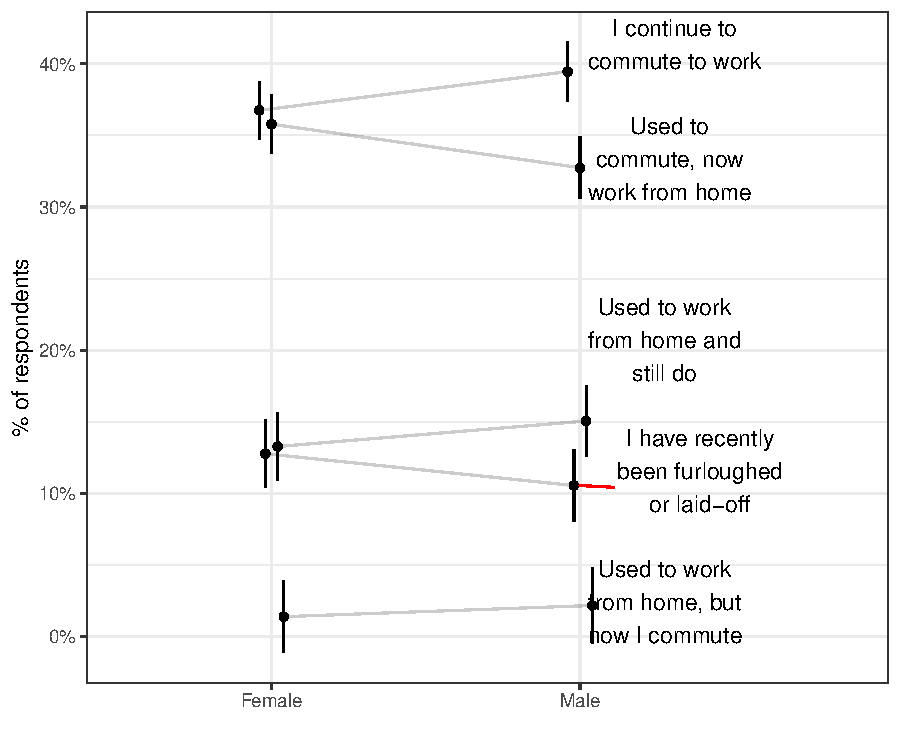
\includegraphics[width = \linewidth]{plots/gender.pdf} \\
  \begin{footnotesize}
    \begin{singlespace}
      \emph{Notes:} Standard errors are reported. 
    \end{singlespace}
    \end{footnotesize}
\end{minipage}
\end{figure} 

\end{document} 
